\subsection{The inner angle of an $n$ convex regular polygon}

% TODO: refactor this.
Suppose a convex polygon with $n$ sides and a center point $S$. Its $n$
consecutive vertices are shown in the figure, namely \(v_1, v_2, v_3, \dots,
v_n\). We observe that

\[
  \text{\large $\Delta$} V_1V_2S \cong \text{\large $\Delta$} V_2V_3S
\]

% Continue here...
This holds true for any pair of consecutive triangles, hence the polygon
is made of $n$ such isosceles triagnles.
That is, $|\measuredangle N_2 N_1 S| = |\measuredangle N_1 N_2 S| \Rightarrow
|\measuredangle N_1 N_2 S| = |\measuredangle S N_2 N_3|$, denoted as \(\beta,
\beta\prime\) respectively.

An angle $\alpha = |\measuredangle N_1 S N_2| = \cfrac{360}{n}$, since such an angle multiplied by $n$ makes for a perfect circle of $360\degree$. 
Likewise $\alpha = 180\degree - 2 \beta$.

% Section II
Let $\phi$ be an inner angle of the polygon, such that $\phi = 2 \beta$ (shown in the figure at the vertex $N_2$).

% Steps of the proof
Given $\alpha$, let us re-arrange the expression in terms of $\beta$:

$$\alpha = 180 - 2 \beta \iff \beta = \cfrac{-\alpha + 180}{2}$$

Knowing the properties of $\alpha$, we substitute $\alpha$ for $\alpha = {360}/n$ and obtain:

$$\beta = \cfrac{-\cfrac{360}{n} + 180}{2} \iff \beta = \cfrac{180n - 360}{2n}$$

Knowing the definition of the inner angle of the polygon, namely $\phi = 2 \beta$, we have that:
$$\phi = 2 \beta = 2 \ast \Bigg( \cfrac{180n - 360}{2n} \Bigg) = \cfrac{180n - 360}{n}$$

The obtained expression can be further simplified to the following:

% End of the proof
$$\phi = \cfrac{(n-2) \pi}{n}$$

$\therefore$ the inner angle of an \textit{n-sided} convex regular polygon is ${(n-2) \ast \pi}n^{-1}$. $\blacksquare$

% Include a picture of a unit circle
% TODO: update the picture to correspond to the updated names. 
\begin{figure}[htp]
    \centering
    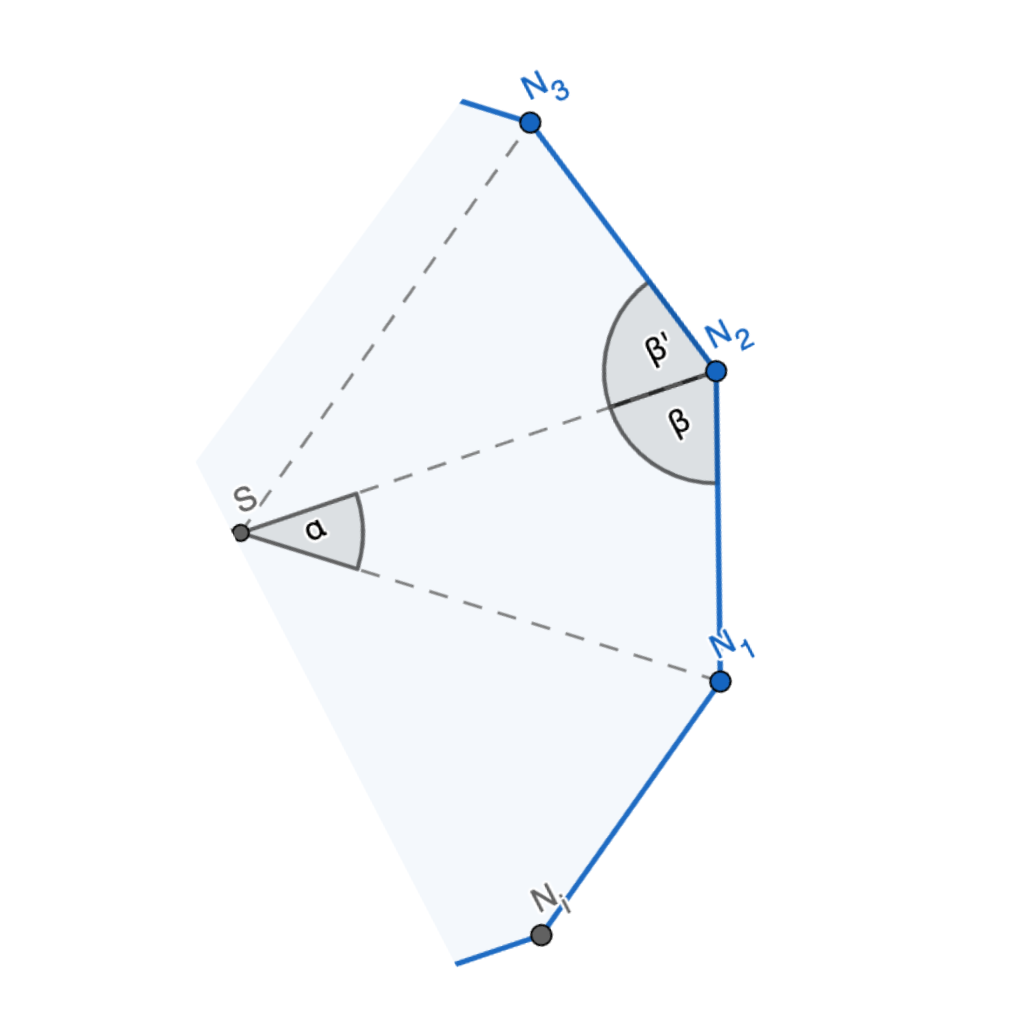
\includegraphics[width=3.cm]{assets/polygon.png}
    \caption{\textit{n-sided} polygon with its 4 vertices in a plane}
\end{figure}
